
\chapter{Fazit \& Empfehlung}
Das Fazit der Arbeit lässt sich in drei Teile Aspekte gliedern. Diese leiten sich aus den Zielen der Arbeit ab, welche in \textbf{\ref{target}} definiert wurden. Es handelt sich dabei um die Aspekte der Sicherheit, der Benutzerfreundlichkeit und der Umsetzbarkeit im Bezug auf einer passwortlosen \ac{SFA}. Das gesamte Fazit dieser Arbeit bezieht sich dabei lediglich auf die passwortlose Authentifizierung mit FIDO2, da die anderen passwortlosen Verfahren nicht weiter betrachtet wurden.

\paragraph*{Sicherheit:} Grundsätzlich handelt es sich bei FIDO2 Protokoll an sich um eine deutlich sicherere Alternative zu einer passwortbasierten Authentifizierung. So übersteigt eine Nutzung von FIDO2 Zugangsdaten auch die Sicherheit einer Nutzung von Passwörtern inklusive \ac{MFA}. Dies liegt insbesondere an der Nutzung von geprüfter asymmetrischer Kryptografie. Es gibt keine geteilten Geheimnisse und der private Schlüssel wird nur lokal auf dem Gerät des Nutzers gespeichert. So werden die meisten Angriffsvektoren der klassischen Passwortauthentifizierung eliminiert. FIDO2 Zugangsdaten lassen sich nicht erraten, phishen und können nicht von Datenlecks betroffen sein. Zudem gilt CTAP2.1 in Verbindung mit WebAuthn als \ac{PQ} bereit. Es handelt sich also auch um eine zukunftsfähige Technologie. Dennoch besteht eine große Abhängigkeit zum genutzten Authentifizierungsgerät. Eine Nutzung von Security Keys führt zu physischen Angriffsvektoren. So kann dieser beispielsweise von Diebstahl betroffen sein. Allerdings lassen sich Security Keys meisten mit einer PIN oder einem biometrischen Merkmal absichern. Dennoch wird die Sicherheit im Vergleich zur passwortbasierten Alternative als höher eingestuft.

\paragraph*{Benutzerfreundlichkeit:} Wie auch im Aspekt der Sicherheit besteht hier eine große Abhängigkeit zum genutzten Authentifizierungsgerät. Grundsätzlich ist FIDO2 in Form von CTAP2.1 und WebAuthn bereits weitreichend verbreitet. Es wird von den meisten Browsern nativ unterstützt und auch Anbieter wie Apple, Microsoft und Google ermöglichen die Nutzung von FIDO2. Nutzer müssen sich keine Passwörter mehr ausdenken und sich diese merken, was einen großen Vorteil darstellt. Dennoch zeigt diese Arbeit auch einige Kritikpunkte auf - insbesondere im Bezug auf die Nutzung von Security Keys. Diese stellen für viele Nutzer eine große Hürde dar. Nutzer kritisierten den Security Key immer bei sich haben zu müssen. Das physische Objekt kann zudem verloren oder kaputt gehen. In solchen Fällen besteht ebenfalls oftmals kein effektiver und sicherer Proezess für eine Wiederherstellung des Zugangs. Auch der entstehende Kostenaufwand und die Verwaltung einer Vielzahl an Security Keys kann im Unternehmenskontext eine Hürde darstellen. Die meisten Nutzer sind zusätzlich so sehr an die Nutzung von Passwörtern gewöhnt, dass es Prozess der Umgewöhnung benötigt wird, um die Akzeptanz zu erhöhen.

\paragraph*{Umsetzbarkeit:} Die Umsetzbarkeit einer Integration von Security Keys mit Hilfe von FIDO2 innerhalb der \ac{LSY} stellt sich in dieser Arbeit als größte Hürde dar. Dies liegt insbesondere an der festen Verankerung der passwortbasierten Authentifizierung in das Sicherheitskonzept und die Richtlinien der \ac{LSY}. Diese zu verändern benötigt einen langen und aufwändigen Prozess. Auch auf technischer Ebene kann sich eine Umstellung in einem so großem Ausmaß als schwierig darstellen. Diese ist aber grundsätzlich möglich und wird von dem Großteil der Systeme unterstützt. Dennoch bestehen auch Sonderfälle, in welchen weiterhin eine Nutzung von Passwörtern notwendig ist. Trotz der weitreichen Unterstützung von FIDO2 ist diese nicht vergleichbar mit der Etablierung von Passwörtern. Dennoch zeigt die Testphase dieser Arbeit auch, dass eine Umstellung der Authentifizierung möglich ist und diese mit einem verhältnismäßig geringen Aufwand umgesetzt werden kann. Mit der aktuellen Umsetzung innerhalb der \ac{LSY} ist eine Nutzung von Security Keys lediglich für eine \ac{MFA} möglich. 

Aus dem Fazit der einzelnen Faktoren wird deutlich, dass FIDO2 insbesondere im Aspekt der Sicherheit viele Vorteile bietet. Auch eine höhere Benutzerfreundlichkeit wird durch FIDO2 grundsätzlich ermöglicht. Hierbei ist allerdings die hohe Abhängigkeit zu den genutzten Authentifizierungsgeräten auffällig. Je nach Auswahl können sowohl Vorteile als auch Nachteile entstehen. In diesem Bereich sollte genauer betrachtet werden, welche Geräte sich in Zukunft etablieren können. Die Ergebnisse dieser Arbeit zeigen, dass die Nutzung von Security Keys noch nicht komplett die ermöglichten Vorteile von FIDO2 ausnutzen können. Auch wenn diese im Bereich der Benutzerfreundlichkeit bereits einige Vorteile bieten, entstehen auch einige Nachteile im Vergleich zu passwortbasierten Alternativen. Eine bessere Variante könnten Passkeys darstellen. Da es sich bei Passkeys allerdings um eine relativ neue Technologie handelt, bleibt ihre Entwicklung abzuwarten. Ein Ausblick zur Nutzung von Passkeys wird in \textbf{\ref{passkeys}} gegeben.

Daraus leitet sich folgende Empfehlung für die Integration einer passwortlosen Authentifizierung innerhalb der \ac{LSY} ab:

Eine Nutzung des FIDO2 Protkolls wird grundsätzlich empfohlen, da dieses eine deutlich höhere Sicherheit bietet und eine höhere Benutzerfreundlichkeit ermöglicht. Allerdings lässt sich noch keine klare Empfehlung für die Nutzung von Security Keys aussprechen. Vielmehr wird empfohlen die Entwicklung der Authentifizierungsgeräte und ihre Verbreitung zu beobachten. Sollte ein Authentifizierungsgerät in der Lage sein die vollen Vorteile auszureizen und weitreichend verbreitet sein, wird eine Nutzung empfohlen. Aus diesem Grund sollte die \ac{LSY} bereits eine Änderung der Richtlinien vornehmen, welche eine Nutzung von FIDO2 ermöglicht. So wird eine signifikant schnellere Handlungszeit ermöglicht. Passwortbasierte Alternativen können weiterhin eingesetetzt werden, könnten aber durch eine vorzeitige Änderung der Richtlininien deutlich schneller ersetzt werden. Zudem würde eine Änderung der Richtlinien eine Testphase in einem größeren Rahmen ermöglichen Dies stellt im Bereich der Umsetzbarkeit aktuell eine große Hürde dar.


\chapter{Ausblick Passkeys} \label{passkeys}
Ein Problem der Nutzung von FIDO2 mit Hilfe von Security Keys ist die Abhängigkeit an ein einzelnes Gerät. Mit Passkeys stellt FIDO Allianz eine Alternative, welche multi-device fähige Zugangsdaten ermöglicht \cite{usecasfido}.
Technisch ist diese Möglichkeit der Authentifizierung bereits in \ac{FIDO}2 integriert. Es besteht allerdings eine Abhängigkeit an die Anbieter der Authentifizierungsgeräte oder Authenticator Apps. Diese müssen die Möglichkeit der Nutzung von Passkeys integrieren \cite{usecasfido}. Dies ist zum aktuellen Zeitpunkt noch nicht weitreichend gegeben.

Die FIDO2-Zugangsdaten werden bei Passkeys nicht auf einem externen Authentifizierungsgerät gespeichert, sondern werden lokal auf dem Gerät selbst gespeichert. Dies führt zu einer deutlich verbesserten Benutzfreundlichkeit im Vergleich zur Nutzung von Security Keys, da keine zusätzliche externe Hardware benötigt wird. Zudem können Passkeys auf mehreren Geräten genutzt werden. So können diese beispielsweise auf einem Smartphone und einem Laptop genutzt werden. Dabei werden die Passkeys zwischen den Geräten synchronisiert (siehe \textbf{\ref{passkeys-img}}). Dies ermöglicht eine Nutzung von Passkeys auf mehreren Geräten. Dadurch besteht allerdings auch eine Abhängigkeit an die Anbieter der Synchronisierungsdienste sowie an Hersteller der Geräte. Diese müssen für die Sicherheit des Betriebssystems, der Hardware und der Synchronisierung sorgen \cite{usecasfido}. 

\begin{figure}[h]
	\centering 
	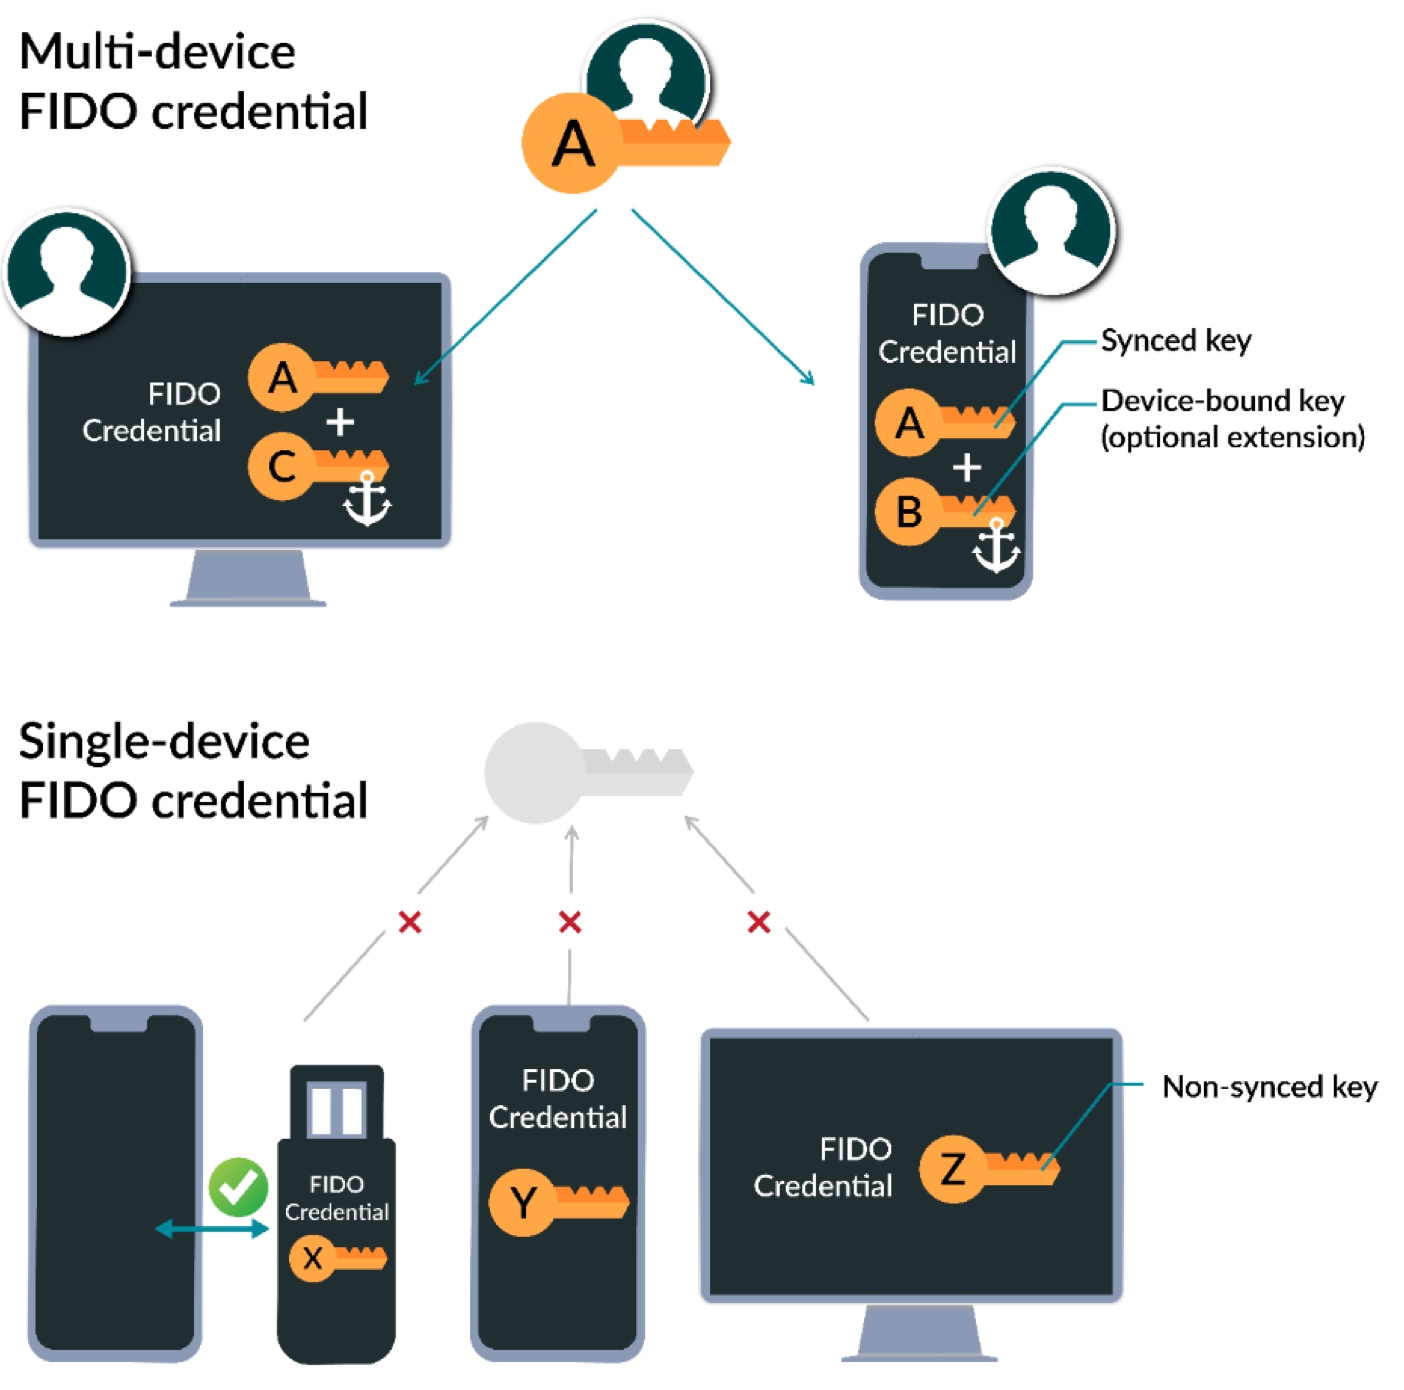
\includegraphics[width=0.7\textwidth]{img/abbildungen/multi-device-fido2.png}
	\captionsetup{format=hang}
	\caption{Multi-device FIDO und Single-device FIDO \cite{usecasfido}} \label{passkeys-img}
\end{figure}

Die Nutzung von Passkeys ist vergleichbar mit der Nutzung von Passwortmanagern, welche ein automatisches Ausfüllen der Zugangsdaten ermöglichen. Dabei bietet die Nutzung von Passkeys allerdings zusätzlich eine erhöhte Sicherheit, selbst ohne eine Nutzung von \ac{MFA} \cite{usecasfido} \cite{passkeysgoogle}. Für die benötigte Autorisierung des CTAP2.1 Standards wird typischerweise ein biometrisches Merkmal des Nutzers genutzt \cite{usecasfido}. Zusätzlich ermöglicht der FIDO2 Standard die Nutzung von Bluetooth. So wird dem Nutzer die Möglichkeit gegeben Passkeys beispielsweise von mobilen Geräten abzurufen. Dies ist eine Absicherung, falls eine Synchronisierung von Passkeys nicht möglich ist oder Geräte die Nutzung von FIDO2 nicht unterstützen. Dies könnte beispielsweise der Fall sein, wenn Geräte unterschiedlicher Anbieter genutzt werden \cite{usecasfido}.

Eine große Authenticator App, welche bereits eine Nutzung von Passkeys unterstützt ist der Google Password Manager. Dieser ermöglich bereits eine verschlüsselte Synchronisierung der Passkeys. Der benötigte private Schlüssel für die Verschlüssellung wird dabei lediglich auf dem Gerät selbst gespeichert und ist dort selbst zusätzlich verschlüsselt \cite{passkeysgoogle}. Google ermöglicht es zudem die Passkeys inklusive eines gerätegebundenen Schlüssels zu nutzen. Dieser Schlüssel wird auf Android Geräten auf der \ac{TEE} gespeichert und ist somit zusätzlich auf der Hardware-Ebene geschützt. Dieser kann das Gerät nicht verlassen und ist ebenfalls nicht durch Backups o.ä. wiederherstellbar \cite{passkeysgoogle}. Der gerätegebundene Schlüssel sorgt für eine erhöhte Sicherheit, da eine Garantie besteht, dass dieser nicht von anderen Geräten genutzt werden kann \cite{usecasfido}. Dies wird auch in \textbf{\ref{passkeys-img}} dargestellt. Dabei handelt es sich um eine optionale Möglichkeit, welche von den Anbietern der Authentifizierungsgeräte oder Authenticator Apps unterstützt werden muss \cite{usecasfido}.

Auch Apple bietet eine synchronisierte Nutzung von Passkeys an. Diese werden dabei in der iCloud Keychain gespeichert. Wie auch bei Google ist dieser dabei ebenfalls lediglich in verschlüsselter Form synchronisiert. Eine Möglichkeit zur Nutzung von Passkeys inkluse eines device-bound Schlüssels wird aktuell nicht in der Dokumentation von Apple erwähnt \cite{passkeysapple}.

Die Entwicklung von Passkeys ist aktuell noch nicht weitreichend und wird nur wenig in der Fachliteratur betrachtet. Es handelt es sich um eine vielversprechende Technologie, welche eine deutlich höhere Benutzerfreundlichkeit ermöglicht. Die Abhängigkeit an die Anbieter der Authentifizierungsgeräte und Authenticator Apps sollte in wissenschaftlichen Arbeiten allerdings noch weiter betrachtet werden. 







